\documentclass[11pt, oneside]{article}

%   ==============================================================================
%   This file is part of the 3D3A MATLAB Toolkit.
%   
%   Contributing author(s), listed alphabetically by last name:
%   Rahulram Sridhar <rahulram@princeton.edu>
%   Joseph G. Tylka <josephgt@princeton.edu>
%   3D Audio and Applied Acoustics (3D3A) Laboratory
%   Princeton University, Princeton, New Jersey 08544, USA
%   
%   MIT License
%   
%   Copyright (c) 2018 Princeton University
%   
%   Permission is hereby granted, free of charge, to any person obtaining a copy
%   of this software and associated documentation files (the "Software"), to deal
%   in the Software without restriction, including without limitation the rights
%   to use, copy, modify, merge, publish, distribute, sublicense, and/or sell
%   copies of the Software, and to permit persons to whom the Software is
%   furnished to do so, subject to the following conditions:
%   
%   The above copyright notice and this permission notice shall be included in all
%   copies or substantial portions of the Software.
%   
%   THE SOFTWARE IS PROVIDED "AS IS", WITHOUT WARRANTY OF ANY KIND, EXPRESS OR
%   IMPLIED, INCLUDING BUT NOT LIMITED TO THE WARRANTIES OF MERCHANTABILITY,
%   FITNESS FOR A PARTICULAR PURPOSE AND NONINFRINGEMENT. IN NO EVENT SHALL THE
%   AUTHORS OR COPYRIGHT HOLDERS BE LIABLE FOR ANY CLAIM, DAMAGES OR OTHER
%   LIABILITY, WHETHER IN AN ACTION OF CONTRACT, TORT OR OTHERWISE, ARISING FROM,
%   OUT OF OR IN CONNECTION WITH THE SOFTWARE OR THE USE OR OTHER DEALINGS IN THE
%   SOFTWARE.
%   ==============================================================================

% Required packages
\usepackage[letterpaper, margin=1in, includeheadfoot]{geometry}
\usepackage{hyperref}
\usepackage{tabularx}

% Header and Footer
\usepackage{fancyhdr}
\pagestyle{fancy}
\renewcommand{\headrulewidth}{1pt}
\lhead{}\chead{\textsc{3D Audio and Applied Acoustics Laboratory $\cdot$ Princeton University}}\rhead{}
\lfoot{}\cfoot{\thepage}\rfoot{}

\renewcommand{\abstractname}{Summary} % Activate to modify the name of the Abstract
%\renewcommand*{\thefootnote}{\fnsymbol{footnote}} % Activate to use symbols rather than numbers for footnotes

% Additional packages
\usepackage{graphicx}
\usepackage{amssymb}
\usepackage{amsmath}
\usepackage[numbers,square,sort]{natbib}
\usepackage{tikz}

% User-defined commands
\newcommand{\citeref}[1]{Ref.~\cite{#1}}
\newcommand{\Citeref}[1]{Reference~\cite{#1}}
\newcommand{\citerefs}[1]{Refs.~\cite{#1}}
\newcommand{\Citerefs}[1]{References~\cite{#1}}
\newcommand{\figref}[1]{Fig.~\ref{#1}}
\newcommand{\Figref}[1]{Figure~\ref{#1}}
\newcommand{\figreftwo}[2]{Figs.~\ref{#1} and~\ref{#2}}
\newcommand{\eqnref}[1]{Eq.~(\ref{#1})}
\newcommand{\eqnreftwo}[2]{Eqs.~(\ref{#1}) and~(\ref{#2})}
\newcommand{\secref}[1]{Section~\ref{#1}}
\newcommand{\Secref}[1]{Section~\ref{#1}}
\newcommand{\secreftwo}[2]{Sections~\ref{#1} and~\ref{#2}}
\newcommand{\secrefthru}[2]{Sections~\ref{#1} through~\ref{#2}}
\newcommand{\tabref}[1]{Table~\ref{#1}}
\newcommand{\Tabref}[1]{Table~\ref{#1}}
\newcommand{\tabreftwo}[2]{Tables~\ref{#1} and~\ref{#2}}
\newcommand{\function}[1]{\paragraph*{\texttt{#1}}}

\begin{document}

% Title and Author block
\begin{centering}
{\Large \textbf{The 3D3A Lab's MATLAB Toolbox}}\\
\vspace{\baselineskip}
\newcolumntype{C}{>{\centering\arraybackslash}p{0.4\textwidth}} % Sets horizontal spacing between authors
\begin{tabular}{CC}
    Rahulram Sridhar & Joseph G.~Tylka \\
    \href{mailto:rahulram@princeton.edu}{rahulram@princeton.edu} & \href{mailto:josephgt@princeton.edu}{josephgt@princeton.edu}
\end{tabular}\\
\vspace{\baselineskip}
v0 -- November 3\textsuperscript{rd}, 2018\\
\end{centering}

% Abstract
\begin{abstract}
The 3D3A lab's MATLAB toolbox is an open-source collection MATLAB functions for spatial audio processing.
In this document, we describe the calculations performed by each of these functions.
\end{abstract}

\section{Introduction}


\section{Function Folders}

%% acoustics %%
\subsection{Acoustics}

\function{f2k} Convert temporal frequency in Hz to angular wavenumber. \\
Computes the angular wavenumber $k$ given temporal frequency $f$, such that
\begin{equation}
k = \frac{2 \pi f}{c},
\end{equation}
where $c$ is the speed of sound in air.

\function{k2f} Convert angular wavenumber to temporal frequency in Hz. \\
Computes the temporal frequency $f$ given angular wavenumber $k$, such that
\begin{equation}
f = \frac{k c}{2 \pi}.
\end{equation}

\function{f2lambda} Convert temporal frequency in Hz to wavelength. \\
Computes the wavelength $\lambda$ given temporal frequency $f$, such that
\begin{equation}
\lambda = \frac{c}{f}.
\end{equation}

\function{getSoundSpeed} Speed of sound in air. \\
Returns the speed of sound in air, given by
\begin{equation}
c = 343~\text{m/s}.
\end{equation}

\function{getPotential} Discrete Fourier transform for acoustic signals. \\
Computes the discrete acoustic potential signal $\psi[k]$ via an $N$-point FFT of an acoustic pressure signal $p[n]$, such that
\begin{equation}
\psi[k] = \frac{1}{N} \sum_{n=1}^N p[n] e^{i 2 \pi (k-1)(n-1) / N}.
\end{equation}

\function{getPressure} Inverse discrete Fourier transform for acoustic signals. \\
Computes the discrete acoustic pressure signal $p[n]$ via an $N$-point IFFT of an acoustic potential signal $\psi[k]$, such that
\begin{equation}
p[n] = \sum_{k=1}^N \psi[k] e^{-i 2 \pi (k-1)(n-1) / N}.
\end{equation}

%% ambisonics %%
\subsection{Ambisonics}

\function{ambSphericalHarmonicY} Real-valued spherical harmonic function. \\
The real-valued spherical harmonics commonly used in ambisonics are given by~\citet[section~2.2]{Zotter2009PhD}
\begin{equation}\label{eq:ambSphericalHarmonicY}
Y_l^m(\theta,\phi) = N_l^{|m|} P_l^{|m|} (\sin \theta) \times
    \begin{cases}
	\cos m \phi & \textrm{for } m \geq 0,\\
	\sin |m| \phi & \textrm{for } m < 0,
    \end{cases}
\end{equation}
where $P_l^m$ is the associated Legendre polynomial of degree $l$ and order $m$, as defined in the MATLAB \texttt{legendre} function\footnote{See:~\url{https://www.mathworks.com/help/matlab/ref/legendre.html}} by
\begin{equation}
P_l^m(x) = (-1)^m (1 - x^2)^{m/2} \frac{d^m}{dx^m} P_l(x), \quad
\textrm{with} \quad
P_l(x) = \frac{1}{2^l l!} \left[ \frac{d^l}{dx^l}(x^2 - 1)^l \right],
\end{equation}
and $N_l^m$ is a normalization term.

\function{ambNormalization} Ambisonics spherical harmonic normalization factor. \\
The orthonormal (N3D) spherical harmonics with Condon-Shortley phase\footnote{Note that including Condon-Shortley phase in the normalization term cancels it in the associated Legendre term.} is given by
\begin{equation}\label{eq:ambNormalization_N3D}
N_l^m = (-1)^m \sqrt{\frac{(2l+1)(2 - \delta_m)}{4 \pi} \frac{(l-m)!}{(l+m)!}},
\end{equation}
where $\delta_m$ is the Kronecker delta.
A commonly-used alternative is the Schmidt seminormalized (SN3D) spherical harmonic normalization convention (again with Condon-Shortley phase), given by~\citep{Nachbar2011}
\begin{equation}\label{eq:ambNormalization_SN3D}
N_l^m = (-1)^m \sqrt{\frac{2 - \delta_m}{4 \pi} \frac{(l-m)!}{(l+m)!}}.
\end{equation}

\function{ambReNormalize} Change normalization of HOA signals. \\
In general, any acoustic pressure signal $x$ may be encoded into ambisonics as a plane-wave source originating from the direction $\hat{r}$ via
\begin{equation}
a_l^m(t) = Y_l^m(\hat{r}) x(t).
\end{equation}
Letting $\tilde{Y}_l^m$ denote the spherical harmonic function with a different normalization, the corresponding ambisonics signal for that normalization is given by
\begin{equation}
\tilde{a}_l^m(t) = \tilde{Y}_l^m(\hat{r}) x(t).
\end{equation}
Consequently, $\tilde{a}_l^m$ is related to $a_l^m$ by
\begin{equation}
\tilde{a}_l^m(t) = a_l^m(t) \frac{\tilde{Y}_l^m(\hat{r})}{Y_l^m(\hat{r})} = a_l^m(t) \frac{\tilde{N}_l^{|m|}}{N_l^{|m|}}.
\end{equation}

%\function{ambNormSquared} Squared norm of the spherical harmonic function. \\
%\begin{equation}
%\| Y_l^m \|^2 = \frac{4\pi}{2l + 1} \left( N_l^0 \right)^2.
%\end{equation}

\function{getACN} Ambisonic channel number (ACN). \\
The ambisonics channel numbering (ACN) convention~\citep{Nachbar2011} is defined such that, for a spherical harmonic function of degree $l \in [0,\infty)$ and order $m \in [-l,l]$, the ACN index $n$ is given by
\begin{equation}\label{eq:getACN}
n = l (l + 1) + m.
\end{equation}

\function{getAmbOrder} Ambisonics order and degree. \\
Correspondingly, for ACN index $n$, the spherical harmonic degree and order are given by
\begin{equation}\label{eq:getAmbOrder}
\begin{aligned}
l &= \left\lfloor \sqrt{n} \right\rfloor,\\
m &= n - l (l + 1),
\end{aligned}
\end{equation}
where $\lfloor \cdot \rfloor$ denotes rounding down to the nearest integer (i.e., the ``floor'' function).

%% auditory
\subsection{Auditory}

\function{fc2erb} Equivalent rectangular bandwidth (ERB) at a center frequency. \\
\citet{GlasbergMoore1990} derived two approximations for the equivalent rectangular bandwidth, given in Hz, as a function of center frequency, given in kHz.
The first approximation is applicable at moderate sound levels and for values of $f_c$ between 0.1 and 10 kHz:
\begin{equation}\label{eq:fc2erb_1}
W_1(f_c) = 24.7(4.37 f_c + 1).
\end{equation}
The second approximation is based on the results of a number of published simultaneous masking experiments and is valid from 0.1 to 6.5 kHz:
\begin{equation}\label{eq:fc2erb_2}
W_2(f_c) = 6.23 f_c^2 + 93.39 f_c + 28.52.
\end{equation}
These two approximations are plotted in \figref{fig:fc2erb}.

\begin{figure}[tb]
    	\centering
    	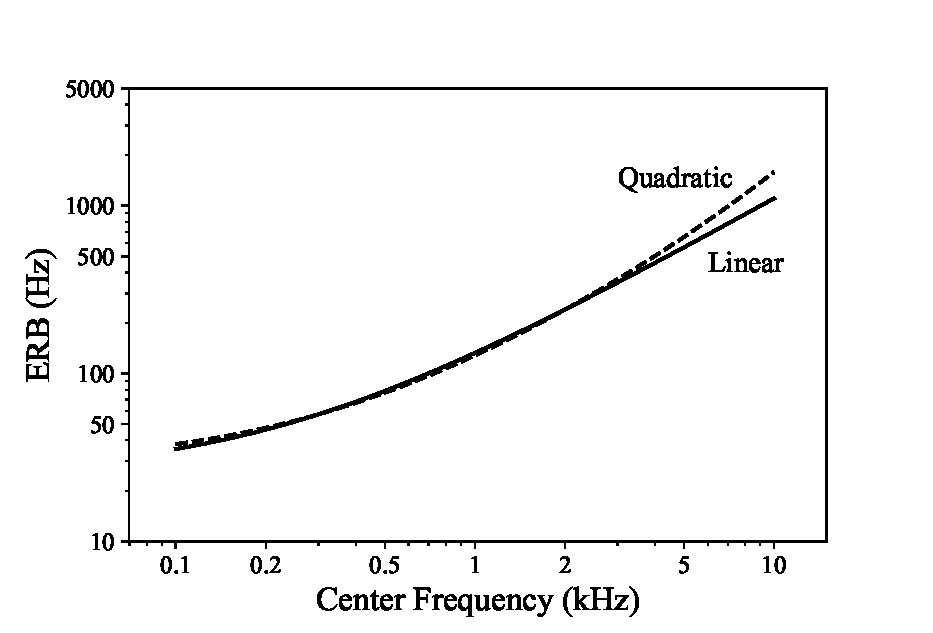
\includegraphics[width=0.55\textwidth]{figures/fc2erb.eps}
    	\caption{ERB approximations of \citet[Fig.~7]{GlasbergMoore1990}.
	The solid curve corresponds to the linear approximation, given in \eqnref{eq:fc2erb_1};
	the dashed curve corresponds to the quadratic approximation, given in \eqnref{eq:fc2erb_2}.}
	\label{fig:fc2erb}
\end{figure}

\function{getGammatoneFilters} Auditory filters that represent human critical bands. \\
This function is essentially a wrapper for the function \texttt{gammatonefir} included in the LTFAT toolbox.
The impulse responses of the gammatone filters are given by
\begin{equation}
g(t) = a t^3 \cos(2 \pi i f_c t) e^{-2 \pi \beta t},
\end{equation}
where, for a sampling rate $F_s$, we have
\begin{equation}
\begin{aligned}
a &= \frac{2 (2 \pi \beta)^4}{3! F_s}, \\
\beta &= 1.0183 \times W_1(f_c),
\end{aligned}
\end{equation}
and $W_1(f_c)$ is the ERB at $f_c$, as given by \eqnref{eq:fc2erb_1}. %%NOTE%% check this

\function{getPattersonFilters} Auditory filters that represent human critical bands. \\
As given by \citet[Eq.~(5.9)]{Salomons1995PhD}, Patterson's auditory filters are given by
\begin{equation}
C(f;f_c) = \left( 1 + \frac{4|f-f_c|}{W_2(f_c)} \right) e^{-\frac{4|f-f_c|}{W_2(f_c)}},
\end{equation}
where $W_2(f_c)$ is the ERB at $f_c$, as given by \eqnref{eq:fc2erb_2}.

%% binaural %%
\subsection{Binaural}

%% dsp %%
\subsection{DSP}

\function{fractionalOctaveSmooth} Fractional-octave smoothing of transfer functions. \\
Used to perform fractional-octave smoothing of a transfer function.
\begin{equation}\label{eq:fractionalOctaveSmooth}
H_\text{s}[k] = \sum_{k' = 0}^{N - 1} M[k, k'] H[k'].
\end{equation}

\function{computeSmoothingMatrix} Fractional-octave smoothing matrix. \\
Used for computing the smoothing matrix $M$.
Currently, the methods of \citet{HatziantoniouMourjopoulos2000} and \citet{Tylka2017} have been implemented.

%% math %%
\subsection{Math}

\function{logmean} Log-scale average of a function. \\
Consider a discrete spectrum $X[k]$ for $k \in [0, K-1]$, where the frequency index, $k$, is proportional to the frequency in Hz, given by $k F_s/K$, and $F_s$ is the sampling rate.
We define the logarithmically-weighted average, $\overline{X}$, over the frequency index range $[K_1, K_2]$, as a weighted average
\begin{equation}\label{eq:logmean}
\overline{X} = \frac{\displaystyle \sum_{k=K_1}^{K_2} \frac{1}{k} \cdot X[k]}{\displaystyle \sum_{k=K_1}^{K_2} \frac{1}{k}}.
\end{equation}

\function{logvar} Log-scale variance of a function. \\
Similarly, we define the logarithmically-weighted variance $\sigma_X^2$ by
\begin{equation}\label{eq:logvar}
\sigma_X^2 = \frac{\displaystyle \sum_{k=K_1}^{K_2} \frac{1}{k} \left( X[k] - \overline{X} \right)^2}{\displaystyle \sum_{k=K_1}^{K_2} \frac{1}{k}}.
\end{equation}

%% metrics %%
\subsection{Metrics}

\function{boren2015\_Epk} Boren's peak and notch errors. \\
Implemented peak and notch errors coloration metrics of \citet{Boren2015}.

\function{computeDirectionalError} Directional error between two vectors. \\
Computes a directional error between two vectors, $\vec{r}_1$ and $\vec{r}_2$, such that
\begin{equation}
\epsilon = \cos^{-1} \left( \hat{r}_1 \cdot \hat{r}_2 \right).
\end{equation}
Alternatively,
\begin{equation}
\epsilon = \sqrt{ \left( \hat{r}_1 - \hat{r}_2 \right) \cdot \left( \hat{r}_1 - \hat{r}_2 \right) }.
\end{equation}

\function{estimateAudibleEnergy} Average energy in auditory critical bands. \\
We define the \textit{mean audible energy} (MAE) of a signal as its average energy in critical bands, i.e.,
\begin{equation}\label{eq:estimateAudibleEnergy}
\text{MAE} = \frac{1}{N_b} \sum_{c = 1}^{N_b} \int_{-\infty}^\infty |\Gamma(f;f_c)| |X(f)|^2 df,
\end{equation}
where $X$ is the Fourier transform of some signal and $\Gamma(f;f_c)$ is the transfer function of a gammatone filter\footnote{In this work, we used the gammatone filters implemented in the large time-frequency analysis toolbox (LTFAT) for MATLAB:~\url{http://ltfat.sourceforge.net/}} with center frequency $f_c$ for $c \in [1, N_b]$, for a set of ERB-spaced (equivalent rectangular bandwidth) center frequencies~\citep{GlasbergMoore1990} spanning the range $f \in [20~\text{Hz}, 20~\text{kHz}]$.

\function{gerzon1992} Gerzon's localization vectors. \\
Implements the velocity and energy vectors of \citet{Gerzon1992}.

\function{kates1984} Kates' central spectrum coloration model. \\
Implements the central spectrum coloration model of \citet{Kates1984}.

\function{merimaa2005} Merimaa's intensity vector and diffuseness parameter. \\
Implements the intensity vector and diffuseness parameter, computed from first-order ambisonics signals, as given by \citet{MerimaaPulkki2005}.

\function{pulkki1999\_CLL} Pulkki's composite loudness level model. \\
Implements the composite loudness level model of \citet{Pulkki1999}.

\function{scharer2009} Scharer's spectral errors in auditory bands. \\
Implements the auditory band spectral error of \citet{ScharerLindau2009}.

\function{stitt2016} Stitt's precedence-effect-based energy vector. \\
Implements the precedence-effect-based energy vector model of \citet{Stitt2016}.

\function{tylka2017} Tylka's precedence-effect localization model for ambisonics. \\
Implements the ambisonics localization vector model of \citet{TylkaChoueiri2017a}.

\function{wittek2007} Wittek's spectral alterations coloration model. \\
Implements the spectral alterations coloration model of \citet{Wittek2007}.

%% stimuli %%
\subsection{Stimuli}

\function{exponentialSineSweep} Generate an exponential sine sweep (ESS). \\
Implements the exponential sine sweep (ESS) of \citet{Farina2000} and the phase-controlled ESS of \citet{VetterdiRosario2011}.

\function{warpedSineSweep} Generate a warped sine sweep. \\
Implements the warped sine sweep of \citet{OchiaiKaneda2013}.

% References
\bibliographystyle{unsrtnat}
\bibliography{refs}

\end{document}